\documentclass{article}
\usepackage{amsmath}
\usepackage{graphicx}
\usepackage[nottoc]{tocbibind}
\usepackage{booktabs}

\title{First Structured Latex}
\date{2013-03-08}
\author{Jean CASSOU-MOUNAT}

\begin{document}

\maketitle
\pagenumbering{gobble}
\newpage
\pagenumbering{arabic}

\tableofcontents

\section{First Section}

Hello World!

\subsection{Introducing math package}

\paragraph{First equation}

\begin{equation*}
  f(x) = x^2
\end{equation*}

\subsection{Second Subsection}

\section{More math with Latex}

\paragraph{Fractions}

\begin{align*}
  g(x) &= \frac{1}{x}\\
  F(x) &= \int^a_b \frac{1}{3}x^3
\end{align*}

\paragraph{Matrix}

\[
 \begin{matrix}
  a & b & c \\
  d & e & f \\
  g & h & i
 \end{matrix}
\]

\section{Picture}

This is a picture about Seoul :

\begin{figure}
  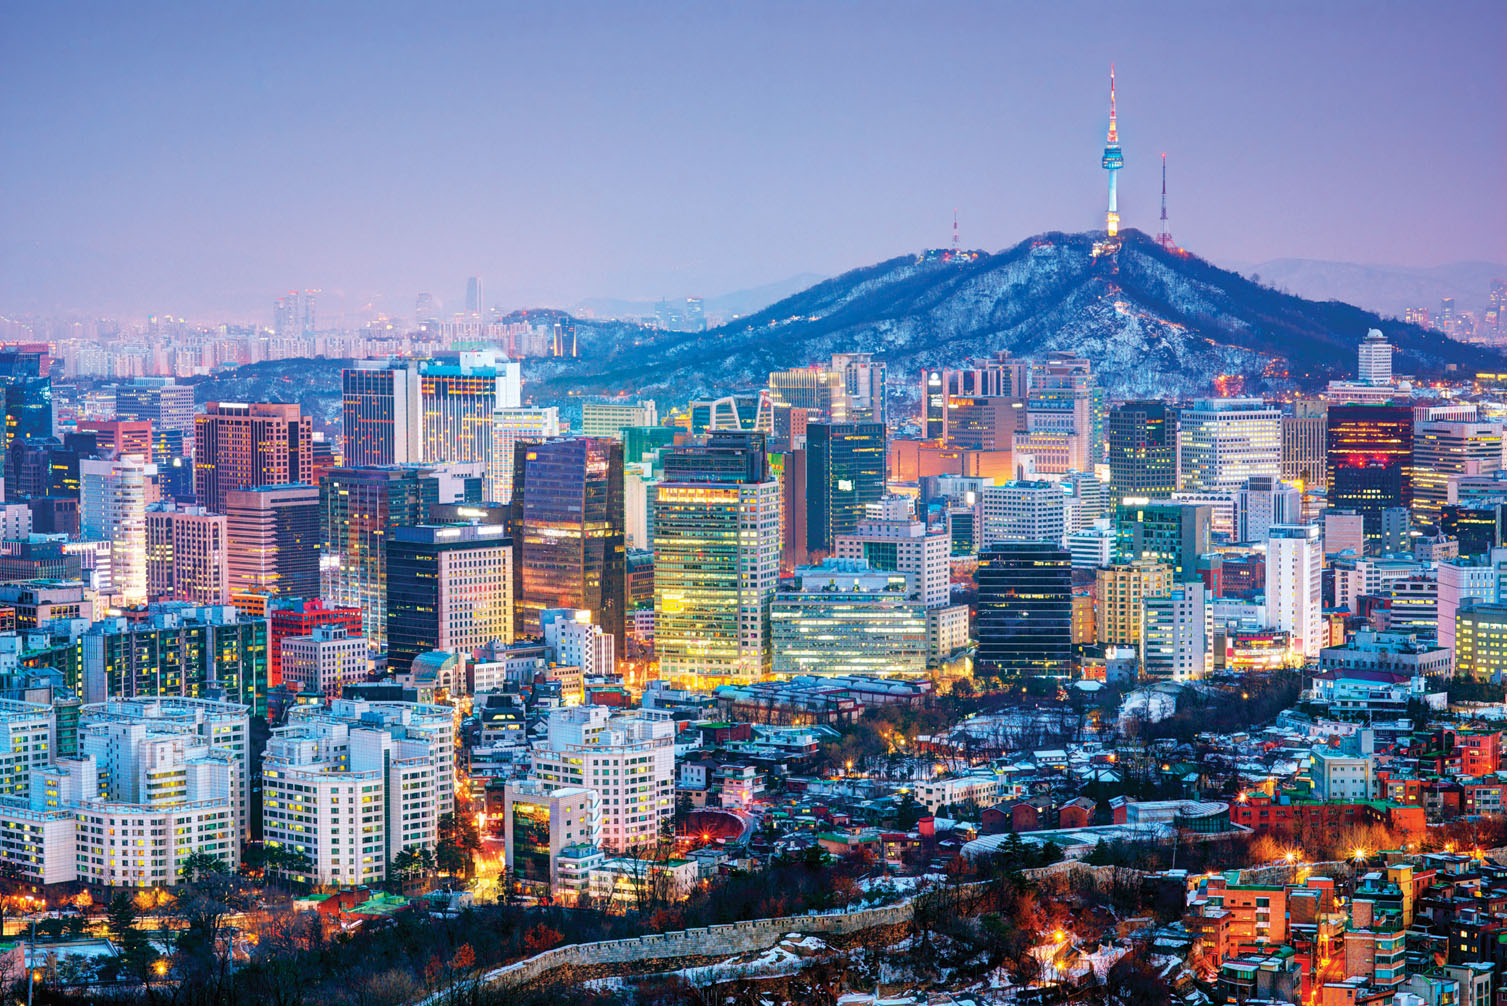
\includegraphics[width=\linewidth]{seoul.png}
  \caption{Seoul}
  \label{fig:seoul1}
\end{figure}

\section{Bibliography}
Three items are cited: \textit{The \LaTeX\ Companion} book \cite{latexcompanion}, the Einstein
journal paper \cite{einstein}, and the Donald Knuth's website \cite{knuthwebsite}. 
The \LaTeX\ related items are \cite{latexcompanion,knuthwebsite}. 
 
\medskip
 
\bibliographystyle{unsrt}
\bibliography{sample}

\section{Footnotes}

This is some example text, but I don't know what this \footnote{\label{myfootnote}This is an old word...} means.

\section{Tables}

\begin{table}[h!]
  \centering
  \caption{Caption for the table.}
  \label{tab:table1}
  \begin{tabular}{ccc}
    \toprule
    Some & actual & content\\
    \midrule
    prettifies & the & content\\
    as & well & as\\
    using & the & booktabs package\\
    \bottomrule
  \end{tabular}
\end{table}

\end{document}

